%%%%%%%%%%%%%%%%%%%%%%%%%%%%%%%%%%%%%%%%%
% Proceedings of the National Academy of Sciences (PNAS)
% LaTeX Template
% Version 1.0 (19/5/13)
%
% This template has been downloaded from:
% http://www.LaTeXTemplates.com
%
% Original author:
% The PNAStwo class was created and is owned by PNAS:
% http://www.pnas.org/site/authors/LaTex.xhtml
% This template has been modified from the blank PNAS template to include
% examples of how to insert content and drastically change commenting. The
% structural integrity is maintained as in the original blank template.
%
% Original header:
%% PNAStmpl.tex
%% Template file to use for PNAS articles prepared in LaTeX
%% Version: Apr 14, 2008
%
%%%%%%%%%%%%%%%%%%%%%%%%%%%%%%%%%%%%%%%%%

%----------------------------------------------------------------------------------------
%	PACKAGES AND OTHER DOCUMENT CONFIGURATIONS
%----------------------------------------------------------------------------------------

%------------------------------------------------
% BASIC CLASS FILE
%------------------------------------------------

%% PNAStwo for two column articles is called by default.
%% Uncomment PNASone for single column articles. One column class
%% and style files are available upon request from pnas@nas.edu.

%\documentclass{pnasone}
\documentclass{pnastwo}

%------------------------------------------------
% POSITION OF TEXT
%------------------------------------------------

%% Changing position of text on physical page:
%% Since not all printers position
%% the printed page in the same place on the physical page,
%% you can change the position yourself here, if you need to:

% \advance\voffset -.5in % Minus dimension will raise the printed page on the 
                         %  physical page; positive dimension will lower it.

%% You may set the dimension to the size that you need.

%------------------------------------------------
% GRAPHICS STYLE FILE
%------------------------------------------------

%% Requires graphics style file (graphicx.sty), used for inserting
%% .eps/image files into LaTeX articles.
%% Note that inclusion of .eps files is for your reference only;
%% when submitting to PNAS please submit figures separately.

%% Type into the square brackets the name of the driver program 
%% that you are using. If you don't know, try dvips, which is the
%% most common PC driver, or textures for the Mac. These are the options:

% [dvips], [xdvi], [dvipdf], [dvipdfm], [dvipdfmx], [pdftex], [dvipsone],
% [dviwindo], [emtex], [dviwin], [pctexps], [pctexwin], [pctexhp], [pctex32],
% [truetex], [tcidvi], [vtex], [oztex], [textures], [xetex]

\usepackage{graphicx}

%------------------------------------------------
% OPTIONAL POSTSCRIPT FONT FILES
%------------------------------------------------

%% PostScript font files: You may need to edit the PNASoneF.sty
%% or PNAStwoF.sty file to make the font names match those on your system. 
%% Alternatively, you can leave the font style file commands commented out
%% and typeset your article using the default Computer Modern 
%% fonts (recommended). If accepted, your article will be typeset
%% at PNAS using PostScript fonts.

% Choose PNASoneF for one column; PNAStwoF for two column:
%\usepackage{PNASoneF}
%\usepackage{PNAStwoF}

%------------------------------------------------
% ADDITIONAL OPTIONAL STYLE FILES
%------------------------------------------------

%% The AMS math files are commonly used to gain access to useful features
%% like extended math fonts and math commands.

\usepackage{amssymb,amsfonts,amsmath}

%------------------------------------------------
% OPTIONAL MACRO FILES
%------------------------------------------------

%% Insert self-defined macros here.
%% \newcommand definitions are recommended; \def definitions are supported

%\newcommand{\mfrac}[2]{\frac{\displaystyle #1}{\displaystyle #2}}
%\def\s{\sigma}

%------------------------------------------------
% DO NOT EDIT THIS SECTION
%------------------------------------------------

%% For PNAS Only:
\contributor{Submitted to Proceedings of the National Academy of Sciences of the United States of America}
\url{www.pnas.org/cgi/doi/xxx}
\copyrightyear{x}
\issuedate{Issue Date}
\volume{Volume}
\issuenumber{Issue Number}

%----------------------------------------------------------------------------------------

\begin{document}

%----------------------------------------------------------------------------------------
%	TITLE AND AUTHORS
%----------------------------------------------------------------------------------------

\title{DOTA} % For titles, only capitalize the first letter

%------------------------------------------------

%% Enter authors via the \author command.  
%% Use \affil to define affiliations.
%% (Leave no spaces between author name and \affil command)

%% Note that the \thanks{} command has been disabled in favor of
%% a generic, reserved space for PNAS publication footnotes.

%% \author{<author name>
%% \affil{<number>}{<Institution>}} One number for each institution.
%% The same number should be used for authors that
%% are affiliated with the same institution, after the first time
%% only the number is needed, ie, \affil{number}{text}, \affil{number}{}
%% Then, before last author ...
%% \and
%% \author{<author name>
%% \affil{<number>}{}}

%% For example, assuming Garcia and Sonnery are both affiliated with
%% Universidad de Murcia:
%% \author{Roberta Graff\affil{1}{University of Cambridge, Cambridge,
%% United Kingdom},
%% Javier de Ruiz Garcia\affil{2}{Universidad de Murcia, Bioquimica y Biologia
%% Molecular, Murcia, Spain}, \and Franklin Sonnery\affil{2}{}}

\author{A. L. Sallaska\affil{1}{The MITRE Corporation},
D. Biro\affil{2}{Albert Einstein College of Medicine},
S. Duran\affil{3}{Pompeu Fabra University},
\and
M. Stuart\affil{4}{University of California, Berkeley}}

\contributor{Submitted to Proceedings of the National Academy of Sciences
of the United States of America}

%----------------------------------------------------------------------------------------

\maketitle % The \maketitle command is necessary to build the title page

\begin{article}

%----------------------------------------------------------------------------------------
%	ABSTRACT, KEYWORDS AND ABBREVIATIONS
%----------------------------------------------------------------------------------------

\begin{abstract}
x\end{abstract}

%------------------------------------------------

\keywords{Keyword1 | Keyword2 | Keyword3} % When adding keywords, separate each term with a straight line: |

%------------------------------------------------

%% Optional for entering abbreviations, separate the abbreviation from
%% its definition with a comma, separate each pair with a semicolon:
%% for example:
%% \abbreviations{SAM, self-assembled monolayer; OTS,
%% octadecyltrichlorosilane}

% \abbreviations{}
\abbreviations{DOTA, Defense of the Ancients}

%----------------------------------------------------------------------------------------
%	PUBLICATION CONTENT
%----------------------------------------------------------------------------------------

%% The first letter of the article should be drop cap: \dropcap{} e.g.,
%\dropcap{I}n this article we study the evolution of ''almost-sharp'' fronts

\section{Introduction}

Existing performance metrics of cyber intrusion detection algorithms, such as false positive or negative rates, are unable to capture the level of granularity necessary to significantly improve the algorithms, especially when a single, definitive outcome is rarely the case for this domain.  Traditional static cyber defense systems also require long lead times to install patch updates, and staving off damage in real time is unfeasible using these metrics.  Therefore, metrics must evolve to provide real-time evaluations of adaptive adversaries whose strategies may change depending on the protective mechanisms they encounter, as well as characterizing sequences of detections.  

Usable data from within the cyber domain that may help to strengthen detection algorithm scoring is nearly nonexistent.  If actual attacks are documented in the real world, this data is rarely made available and may be network specific (hence, not generalizable).   Thus, a proxy for the data is necessary.  An online battle arena video game called Defense of the Ancients 2 (DOTA 2) is a rich data source of real-time adaptive adversaries.  DOTA 2 is a strategic, competitive, multiplayer game where two teams of five individuals each compete against each other to complete objectives and to destroy the other team?s base in a time frame of $\sim$ 20 to $\sim$ 90 minutes.  The players deploy various in-game and between-game tactics and procedures to achieve a specific measurable objective.  Professional players vie for tens of millions of dollars in prize pools each year, and over 2 billion games have been played.  The results in this paper are using data from a cache of 500 GB of aggregated game data ($\sim$ 2.5 million games played over one year) and from X GB of raw, event-by-event data.  Our goal is to use this data to shed light on how we can 1) detect and 2) quantify the rate of change of strategies in co-evolutionary systems.  

This is akin to the classic `Red Queen hypothesis' in evolutionary biology, but in this case we are interested in human behaviors where a strategy can be considered most generally as a `meme' of sorts.  Our hypotheses include: 1) a mapping exists between game observables and a set of strategies, 2) a measurable signal can be extracted from which to ascertain the adoption, stabilization, and decay of specific strategy traits, 3) changes in strategies occur over time, and 4) strategy changes are driven (at least in part) from behaviors of the opposing team.  We postulate that testing these hypotheses will require an understanding of the co-evolutionary dynamics of the overall environment.  In particular, the human behavioral components underlying the adversary/defense team actions will need to be assessed.  The use of data from a multiplayer online game for this purpose assumes there is a valid mapping between the `game-space' to `cyber-space' behaviors from which useful inferences can be made.  Through this exercise we hope to understand what types of data (if any) are useful for this purpose and how one might develop proxies to characterize strategies.  Ultimately, we hope that the analysis could be applied against realistic data specific to a cyber intrusion.  

\section{The Game: DOTA 2}

An aerial view of the DOTA game board is shown in Fig.~\ref{gameboard}.  The goal of the game is to destroy the opposing team's base, their Ancient, located either in the lower left or upper right corner of the figure.  

\begin{figure}[h]
\centerline{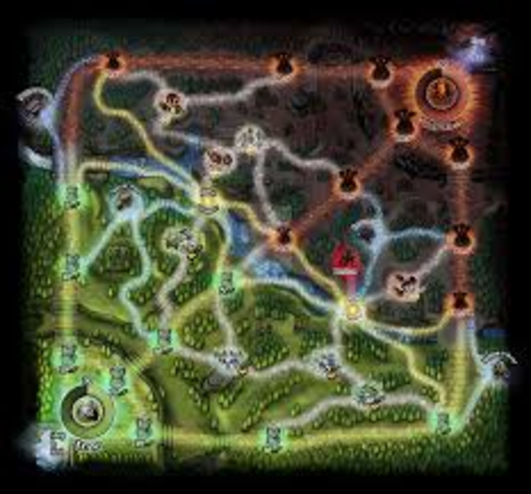
\includegraphics[width=0.8\linewidth]{./Figs/GameBoard.pdf}}
\caption{Game board of DOTA 2.}\label{gameboard}
\end{figure}

Ten human players are divided into two teams of five (the Dire and the Radiant teams), each controlling a `hero' character, which is chosen via a drafting process in professional games (discussed in more detail in the following section).  Each hero has its own set of unique abilities and is generally divided into one of three categories: intelligence, strength, or agility.  Throughout the game, the heroes amass 1) experience (XP) in order to become more powerful and unlock special abilities and 2) gold in order to buy items which also increase power.  

There are three main `lanes' to reach each Ancient, along the outer edges and down the diagonal.  There is also a jungle landscape between the lanes.  Various computer-controlled characters called `creeps' are deployed throughout the game which allow heroes to gain experience.  Defensive towers also line the lanes and protect the Ancient against enemy heroes.  

\subsection{The Draft}

Heroes are chosen from a pool of $\sim$ 120 characters.  In professional games, there are twenty choices for ten human players, five hero picks and five hero bans for each team, chosen in the following order:
\\
\\
B1 B2 B1 B2 P1 P2 P2 P1 B1 B2 B1 B2 P2 P1 P2 P1 B2 B1 P2 P1
\\
\\
where B indicates a ban, P indicates a pick, and the number refers to the team.  



\section{Analysis and Results}

\subsection{Draft}

\subsubsection{Salva} 

\subsubsection{Dan}


\subsection{Within Game (Anne)}

The raw game data is initially downloaded from a DOTA 2 repository in a binary form.  A java parser was written to convert the data into a JSON format, with each event occurring in the game generating an output.  An example for a hero movement event is shown below:
\\
\\
\{``tick":24516,``time":825,``type":``DT\_DOTA\_Unit\_Hero\_Omniknight", ``team":3,``x":99,``y":171\}
\\
\\
where `tick' is a subunit of `time', and team indicates 2 or 3 (which must be connected with Dire or Radiant, see below).  The type of event includes position, items, abilities, gold, XP, damage, healing, and death, with each type triggering different tags following the type.  This event-by-event data, which can include multiple events per time step, was transformed into a single time step which keeps track of all events occurring at that step for each hero on each team.  Aggregated statistics for the game a whole, such as which team won and draft order, was folded in with this event data.  The draft order from the aggregated statistics allows the hero names and team number (2 or 3) to be correlated with each team, Dire or Radiant, as the Radiant are denoted as team 0 in the draft.  This is important as the win is denoted as a boolean value for if the Radiant team won or lost, not if team 2 or 3 won or lost.  


\begin{figure}[h]
\centerline{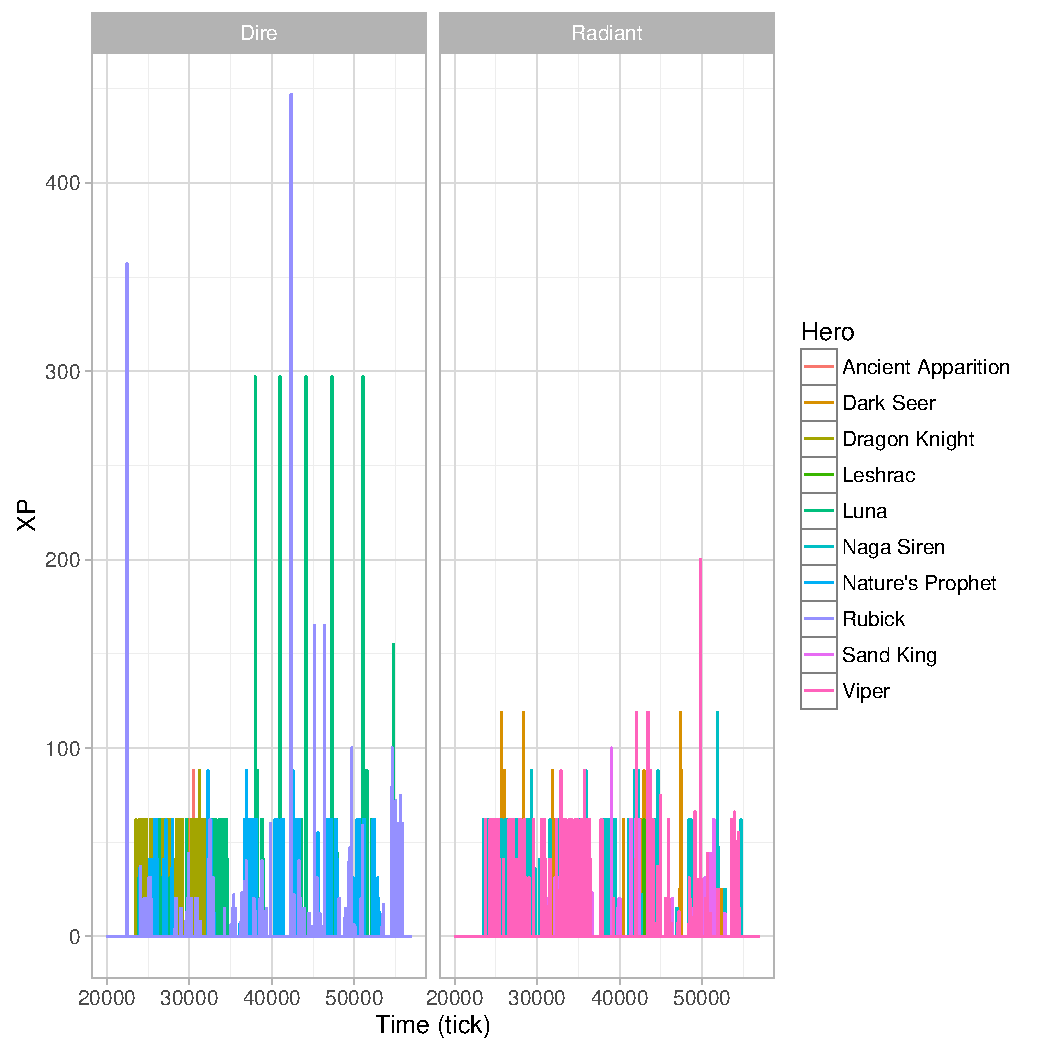
\includegraphics[width=0.8\linewidth]{./Figs/XP_example.pdf}}
\caption{Game board of DOTA 2.}\label{gameboard}
\end{figure}






\subsection{Between Games (Marla)}


%----------------------------------------------------------------------------------------
%	APPENDICES (OPTIONAL)
%----------------------------------------------------------------------------------------

\appendix
An appendix without a title.

\appendix[Appendix title]
An appendix with a title.

%----------------------------------------------------------------------------------------
%	ACKNOWLEDGEMENTS
%----------------------------------------------------------------------------------------

\begin{acknowledgments}
x
\end{acknowledgments}

%----------------------------------------------------------------------------------------
%	BIBLIOGRAPHY
%----------------------------------------------------------------------------------------

%% PNAS does not support submission of supporting .tex files such as BibTeX.
%% Instead all references must be included in the article .tex document. 
%% If you currently use BibTeX, your bibliography is formed because the 
%% command \verb+\bibliography{}+ brings the <filename>.bbl file into your
%% .tex document. To conform to PNAS requirements, copy the reference listings
%% from your .bbl file and add them to the article .tex file, using the
%% bibliography environment described above.  

%%  Contact pnas@nas.edu if you need assistance with your
%%  bibliography.

% Sample bibliography item in PNAS format:
%% \bibitem{in-text reference} comma-separated author names up to 5,
%% for more than 5 authors use first author last name et al. (year published)
%% article title  {\it Journal Name} volume #: start page-end page.
%% ie,
% \bibitem{Neuhaus} Neuhaus J-M, Sitcher L, Meins F, Jr, Boller T (1991) 
% A short C-terminal sequence is necessary and sufficient for the
% targeting of chitinases to the plant vacuole. 
% {\it Proc Natl Acad Sci USA} 88:10362-10366.


%% Enter the largest bibliography number in the facing curly brackets
%% following \begin{thebibliography}

\bibliography{}
\bibliographystyle{unsrt}

%----------------------------------------------------------------------------------------

\end{article}

%----------------------------------------------------------------------------------------
%	FIGURES AND TABLES
%----------------------------------------------------------------------------------------

%% Adding Figure and Table References
%% Be sure to add figures and tables after \end{article}
%% and before \end{document}

%% For figures, put the caption below the illustration.
%%
%% \begin{figure}
%% \caption{Almost Sharp Front}\label{afoto}
%% \end{figure}


%% For Tables, put caption above table
%%
%% Table caption should start with a capital letter, continue with lower case
%% and not have a period at the end
%% Using @{\vrule height ?? depth ?? width0pt} in the tabular preamble will
%% keep that much space between every line in the table.

%% \begin{table}
%% \caption{Repeat length of longer allele by age of onset class}
%% \begin{tabular}{@{\vrule height 10.5pt depth4pt  width0pt}lrcccc}
%% table text
%% \end{tabular}
%% \end{table}

%\begin{table}[h]
%\caption{Table caption}\label{sampletable}
%\begin{tabular}{l l l}
%\hline
%\textbf{Treatments} & \textbf{Response 1} & \textbf{Response 2}\\
%\hline
%Treatment 1 & 0.0003262 & 0.562 \\
%Treatment 2 & 0.0015681 & 0.910 \\
%Treatment 3 & 0.0009271 & 0.296 \\
%\hline
%\end{tabular}
%\end{table}

%% For two column figures and tables, use the following:

%% \begin{figure*}
%% \caption{Almost Sharp Front}\label{afoto}
%% \end{figure*}

%% \begin{table*}
%% \caption{Repeat length of longer allele by age of onset class}
%% \begin{tabular}{ccc}
%% table text
%% \end{tabular}
%% \end{table*}

%----------------------------------------------------------------------------------------

\end{document}